\chapter{Architecture} \label{chap:Architecture}
To build Offroads, many technologies needed to be harnessed in order to produce the features needed for the Trail Running Website. In \autoref{chap:TrailInterface} we discussed the interface used to create and display trails, in this chapter we discuss how we provide this interface to the user with our chosen \Gls{frontend} framework in \autoref{sec:frontendFramework}. We discuss the extra features needed that the web application provides in \autoref{sec:ExtraFeatures}.

\section{Overview}
The client of the web application (including the trail interface described in chapter \ref{chap:TrailInterface}) are created with Angular. The client sends to and retrieves data from a GraphQl Server. The GraphQl Server is connected to a MySQl database. Prisma provides a GraphQl \acrfull{dal} to simplify access to the data stored in the database. This overall structure can be seen in \autoref{fig:graphArchitecture}.

\begin{figure}[htb!]
    \centering
    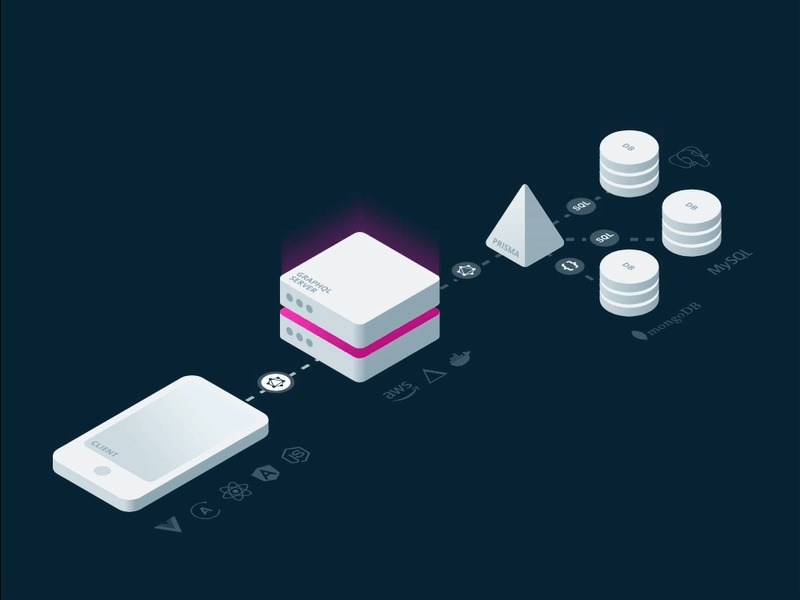
\includegraphics[width=\textwidth]{graphql-architecture.jpg}
    \caption{Overall Architecture of the web application}
    \label{fig:graphArchitecture}
\end{figure}

Our server responds with data written in \acrfull{json} format.

\section{GraphQL Backend}
GraphQL supports 3 main operations
\begin{itemize}
    \item Queries: reading data (analogous to GET requests from \acrshort{rest})
    \item Mutations: modifying data (analogous to POST and PUT request from \acrshort{rest}), and,
    \item Subscriptions: subscribing to real-time changes to data.
\end{itemize}

Whenever the client sends any of the above operations, the client also defines the shape of the data it wants to be returned. This then has to be parsed by the GraphQL who uses resolver functions to retrieve the data the client requests for and stitches them in the shape requested. This allows for a GraphQl server to have multiple data sources.

\subsection{GraphQL resolver functions}
GraphQL executes the query in the shape \cite{jonas2016graphql}. It first executes the root query and then traverses down the tree of the structure defined by the user, calling all the resolver functions needed to return the data required (see \autoref{fig:graphQlResolver}.


\begin{figure}[htb!]
    \centering
    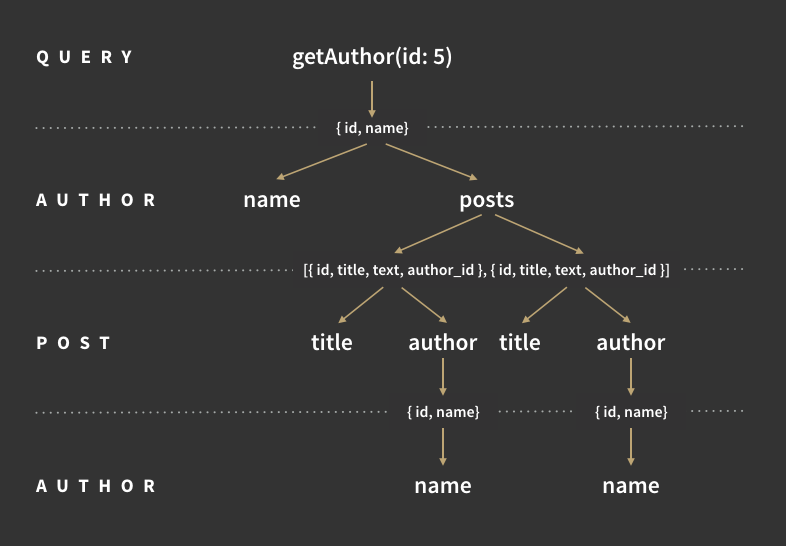
\includegraphics[width=\textwidth]{graphql-resolver.png}
    \caption{GraphQL resolver function}
    \label{fig:graphQlResolver}
\end{figure}

This benefit to the client comes with its own complexities. As we use an SQL database, having to write queries for each resolver function that needs to be called can become counter intuitive to the advantages provided. This is why we use Prisma as a \acrfull{dal} between our server and our database.

\subsection{Prisma Layer}
Prisma\footnote{\url{https://www.prisma.io/}} is a data access layer that replaces traditional \acrfull{orm}. It sits in front of databases and provides methods that allow the server to access the database. The main feature that it provides is the Prisma Client, which is an auto-generated type-safe database client that creates the data access layer. Rather than having to write the SQL queries, Prisma reads our GraphQL schema and uses that to generate functions we can use to access our database (see \autoref{fig:prismaGenerate}).

\begin{figure}[htb!]
    \centering
    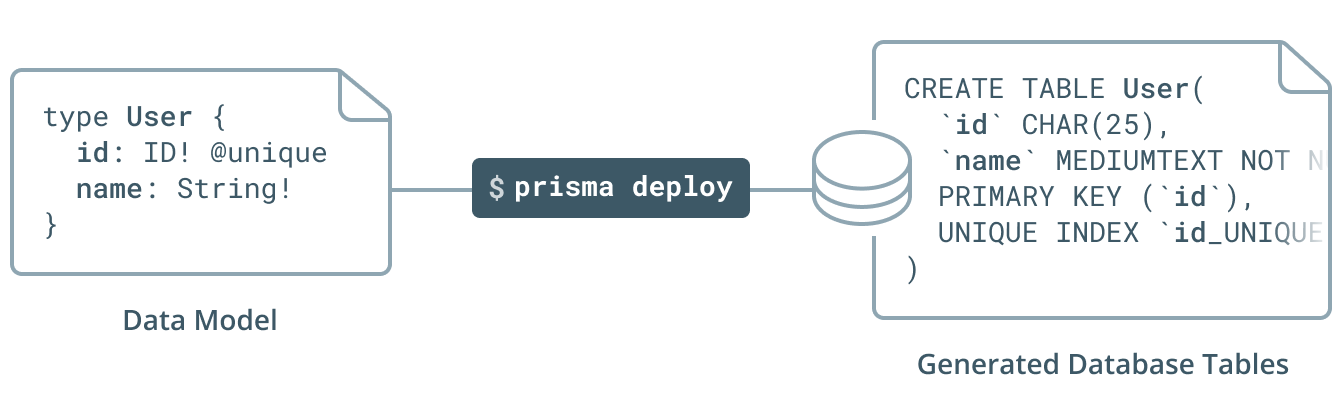
\includegraphics[width=\textwidth]{prisma-generate.png}
    \caption{Prisma generated sql}
    \label{fig:prismaGenerate}
\end{figure}


\section{Frontend Framework} \label{sec:frontendFramework}
There are 2 main way's to build modern web applications. It can be done using native web stack of HTML, CSS and JavaScript or (and more popularly), built using modern web application frameworks. Although there are many proponents to building with the native web stack, modern applications, such as this one, are more complex in nature and hence, require tools make it easier to build complex solutions. They also have big communities and strong documentation that make debugging easier \cite{medium:WhyModernJSFrameworkExist}.

There are a large variety Frontend Frameworks out there. I considered the most popular ones which where
\begin{itemize}
    \item Angular \footnote{\url{https://angular.io/}}
    \item React \footnote{\url{https://reactjs.org/}}
    \item Vue.js \footnote{\url{https://vuejs.org/}}
\end{itemize}

The framework I decided on was Angular. This was because it has excellent and well-detailed documentation, it came out of the bag with all most of the tools I needed to get started with, and it used Typescript over JavaScript.

Typescript \footnote{\url{https://www.typescriptlang.org/}} is a super set \footnote{it is built on top of JavaScript} of JavaScript, created by Microsoft that provides optional but strict type checking, making developing large scale applications easier \cite{bierman2014understanding}. It also allows me to combine JavaScript's functional programming paradigm \cite{hughes1989functional}, with an Object oriented programming paradigm.

\subsection{State Management With Redux}
One of the main problems that comes with building web applications is managing state in the frontend. On the editor page, where user's create and trails, It is important to manage the state of the application to allow users to undo and redo any changes they make when creating or editing Trails.

It is possible to create your own system to manage state in angular using systems such as Angular's Dependency Injection \cite{wiki:DependencyInjection}, however this does not suffice to handle applications with many interactions. It also doesn't provide standard support for recording user interactions and a means of replaying those steps when needed.

Redux is JavaScript library created by Facebook use for managing state in user interfaces \cite{wiki:Redux}. NgRx \cite{cheng2018state} is a framework built on the fundamentals of Redux\footnote{The Flux Architecture}, to enable us to maintain state in our Application. It is provides a functional way of building Reactive Applications.

With NgRx we can easily manage and control the state of our web application. This is especially useful in on the editor page, where users can create trails described in \autoref{chap:TrailInterface}. With NgRx, we can easily provide undo and redo features. It is common for users to make mistakes when creating a trail, hence allowing users to undo and redo actions they've performed would be hugely beneficial. NgRx helps us manage the state tree (shown in \autoref{fig:reduxStateTree}) of our application in the form of a stack, including the actions users use to create trails. This allows us to traverse the stack of the users actions allowing for redoing and undoing.

\begin{figure}[htb!]
    \centering
    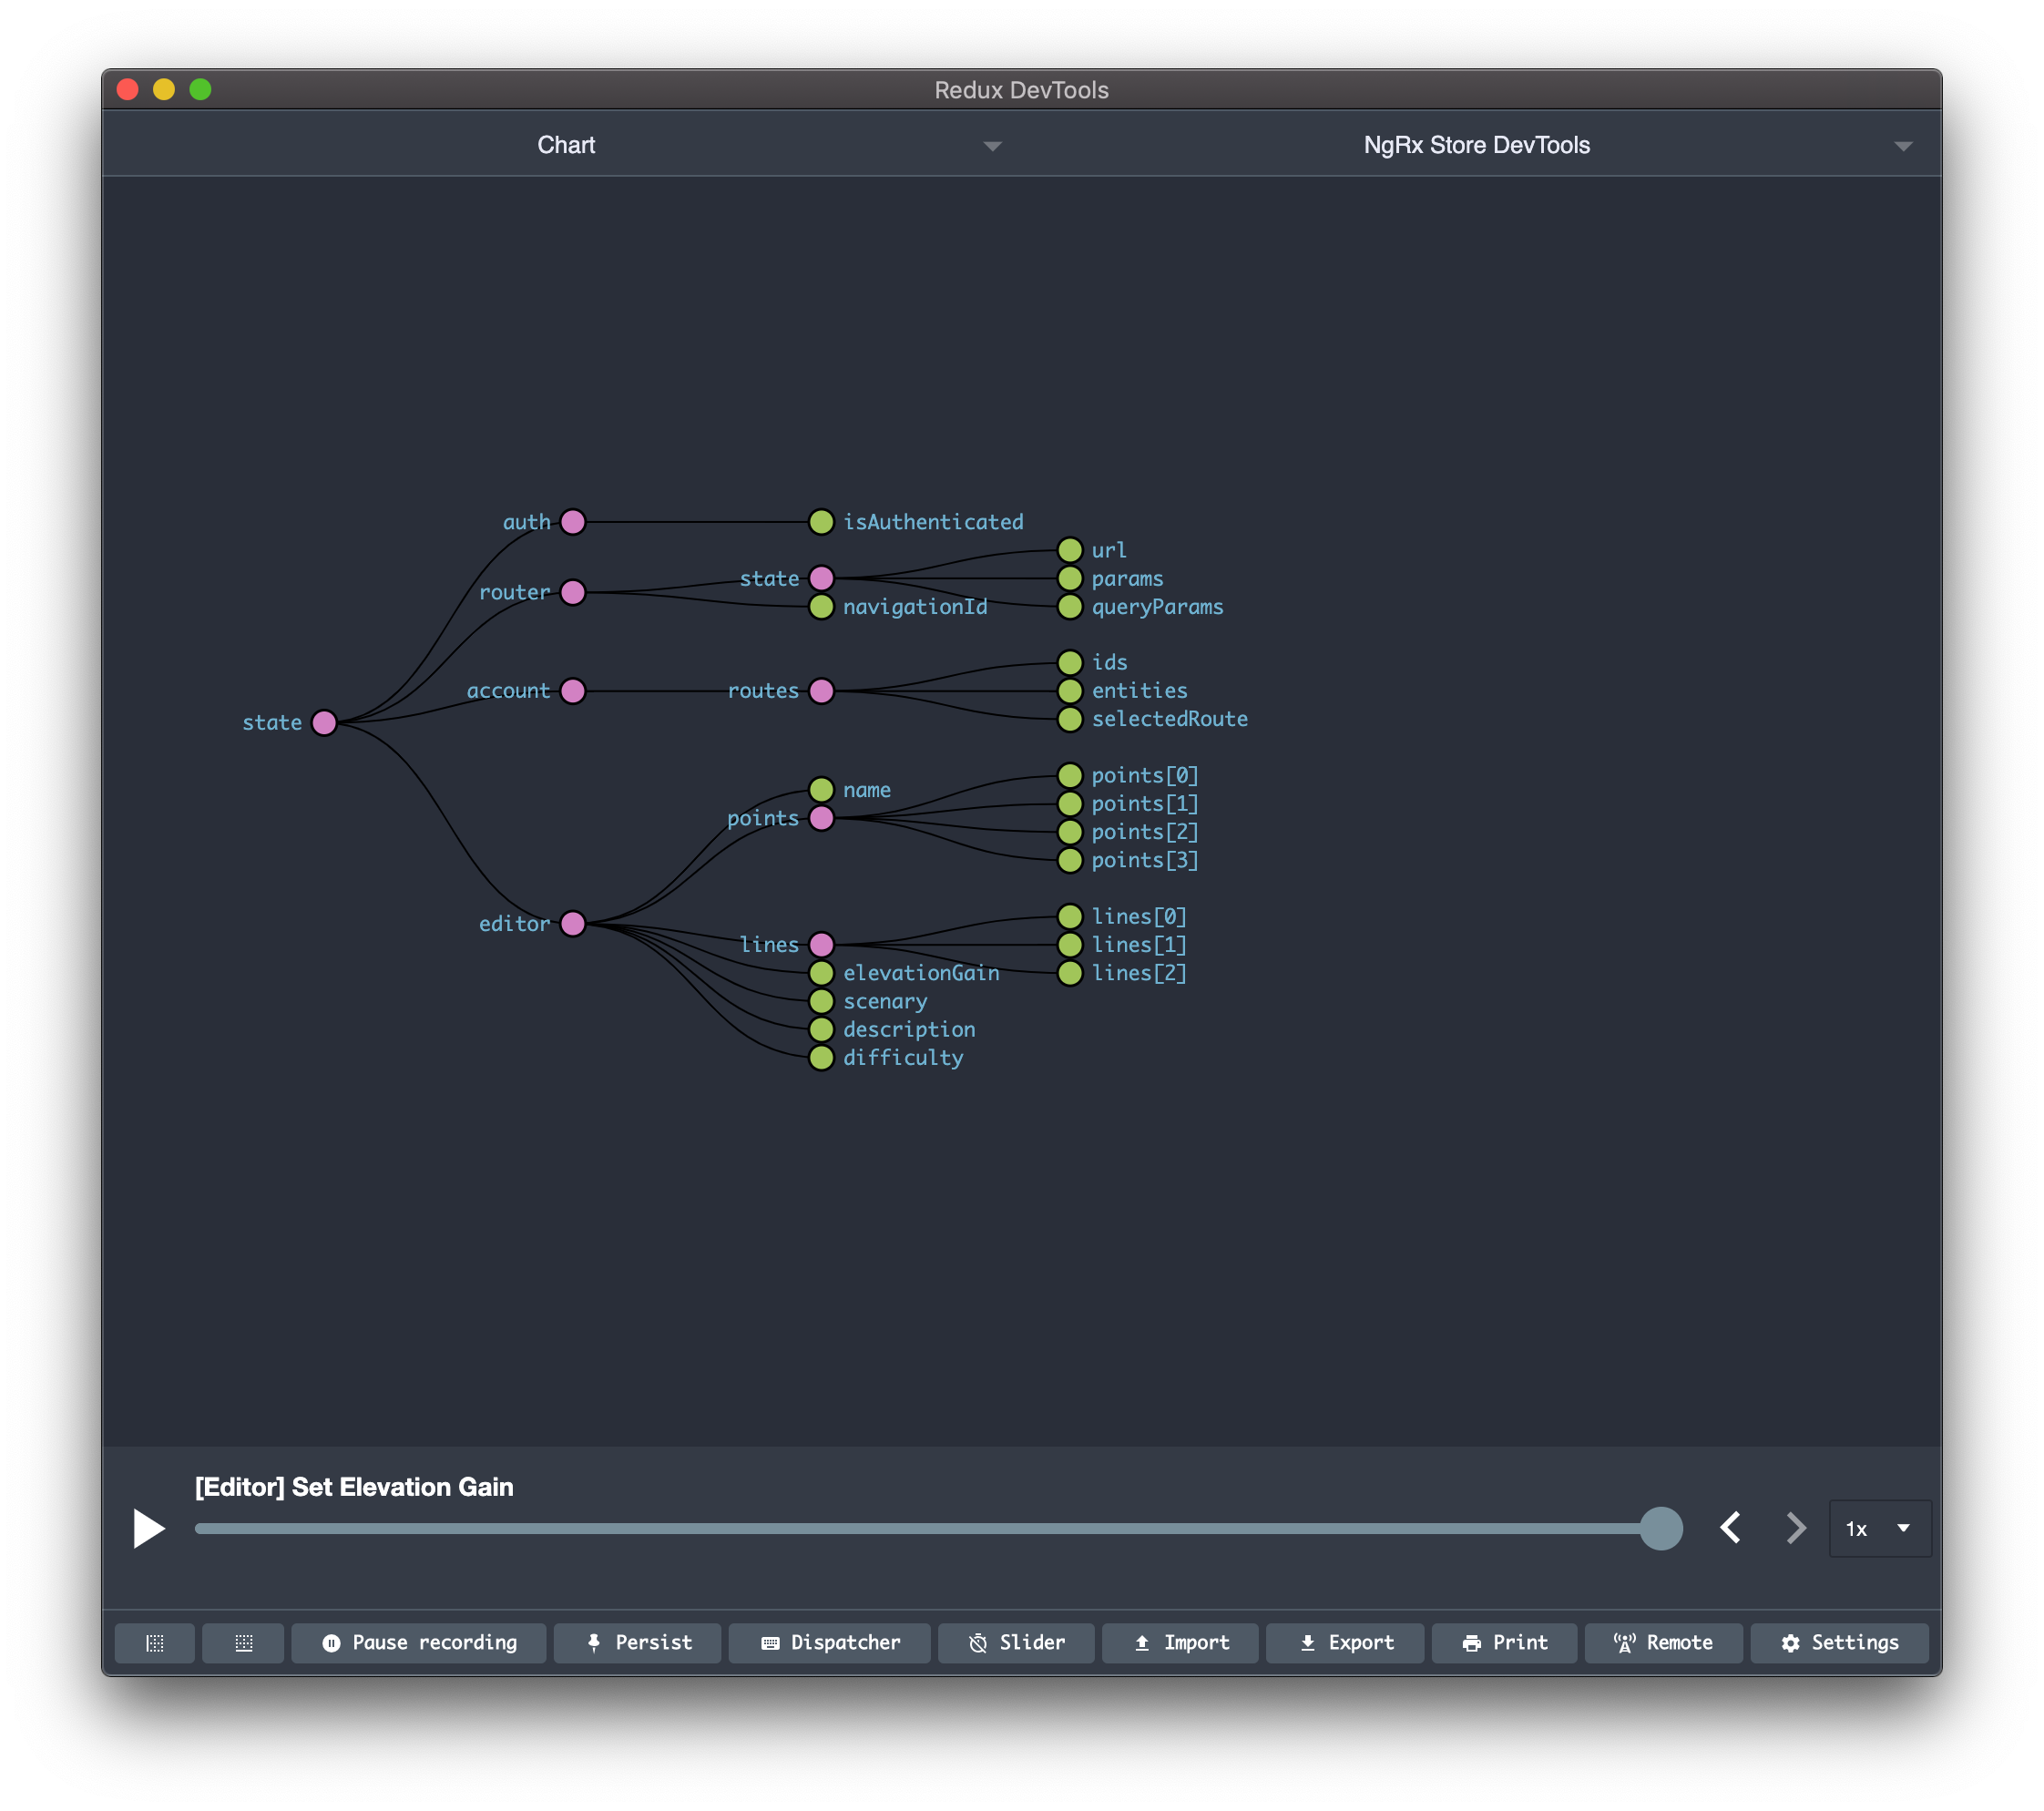
\includegraphics[width=\textwidth]{ngrx-state-tree.png}
    \caption{Redux State tree}
    \label{fig:reduxStateTree}
\end{figure}

\section{Authentication and Authorisation}
Authentication, Authorisation  are a crucial part of Identification any web application s to ensure the users can only interact data intended for them. Moreover, it is needed to allow users to be able to login to the system. The system provides authentication and authorisation with the power of \acrfull{jwt}.

\acrshort{jwt} is a compact open standard (RFC 7519), that allows the secure transmission of tokens between two parties in  \acrshort{json} format \cite{jones2015json}. The information shared between the two parties is digitally signed, and hence can trusted between be verified and trusted by the parties \cite{auth02019json}. This gives us a lightweight way of providing authentication and authorisation between the client on our user and the server.

Each user has a unique email they add when they sign-up as defined in our schema seen in appendix \ref{app:graphqlSchema}. When a user, attempts to log in with their email (which is unique to each user) we find the user in the database and their user ID. Once the Id is found we digitally sign the user ID using the standard \acrfull{hs256} and a secret. As the system is the only one that knows the secret, this ensures integrity. This token is then sent the the client and the client can store this token locally.

Whenever the client needs to authorise themselves, the client sends the request information (such as a query) and the token as part of the Authorisation header. The server reads the token from the header and can use that to verify client, granting them authorisation when needed.

\section{Necessary CRUD operations} \label{sec:ExtraFeatures}
\acrfull{crud} are the four basic operations that most web applications need to provide \cite{codeacademy2019crud}. They are self explanatory verbs that provide the essential operations user's need to be able to interact with web applications.

\subsection{Uploading a Trail}
When a user creates a trail using the map interface described in \autoref{chap:TrailInterface}, it is persisted to the server to be stored in the database. The information needed to be stored for trails are the name of the trail (for identification and searching), points and the lines that are used to create the trail (including the elevation and distance information). We store the points and lines to be used to redraw the trail on the map interface when presenting it to the user. A user can have multiple created trails

\subsection{Exploring Trails}
Exploring trails is how users can find new trails. The main way users can explore trails is via the Recommender system discussed in \autoref{chap:Recommender}. The system also provides other methods to allow users to find trails.

\subsubsection{Sorted Ranked List of Trails}
On the main explore page, there are tabs displaying trails in sorted ranked list. Although in \autoref{subsec:WhyRecSystems}, we discuss the importance of using Recommender systems to suggest trails, the Recommender system is slightly ineffective with new users who are yet to run a trail. Hence we provided other methods of ranking trails to the user.

\begin{itemize}
    \item \textbf{Popular trails:} Trails sorted in descending order of the number of users who run the trail (i.e. trails with the most runs are ranked at the top). 
    \item \textbf{Top rated trails:} Trails sorted in descending order of the average rating from users who run the trail.
    \item \textbf{Recently added trails:} Trails sorted in descending order of the date they where created.
\end{itemize}

\subsubsection{Real time Search}
Users should also be able to search for specific trails and users. The system offers the capability of real time searches of trails and users. To do this, they server will need to be queried as the user types in the search string, creating a performance bottleneck. Angular comes built in with a technology called RxJs that allows us to alleviate this bottleneck.

RxJs is a Javascript library from ReactiveX built on the Reactive programming paradigm \cite{wan2000functional}. It's an API for asynchronous programming with observable streams \cite{reactivex2018main}. It allows us to treat our user input as data streams, that we can subscribe to and manipulate before sending the request to the server. ReactiveX provides us with operators to help improve the efficiency of our real time search. There are 2 main operators that help us do this.

\paragraph{Debounce time} seen in \autoref{fig:debounceTime} only emits values at certain time intervals and discard values that take less than the set interval \cite{leanrrxjs2019debounce}. This prevents us from sending requests every keystroke and as we debounce time in milliseconds, the user does not notice.

\begin{figure}[htb!]
    \centering
    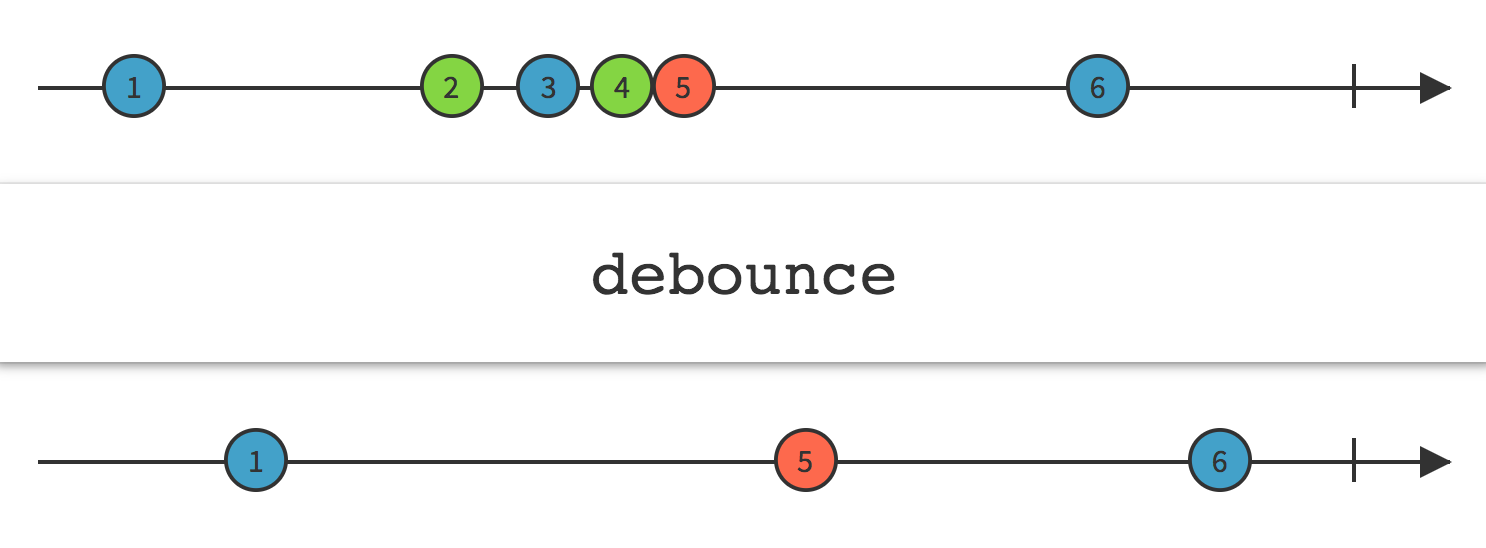
\includegraphics[width=\textwidth]{debounce-time.png}
    \caption{Debounce Time Operator}
    \label{fig:debounceTime}
\end{figure}

\paragraph{Distinct until changed} seen in \autoref{fig:distinctUntilChanged} only emits the current value if it is different from the previous value \cite{leanrrxjs2019distinct}.
\begin{figure}[htb!]
    \centering
    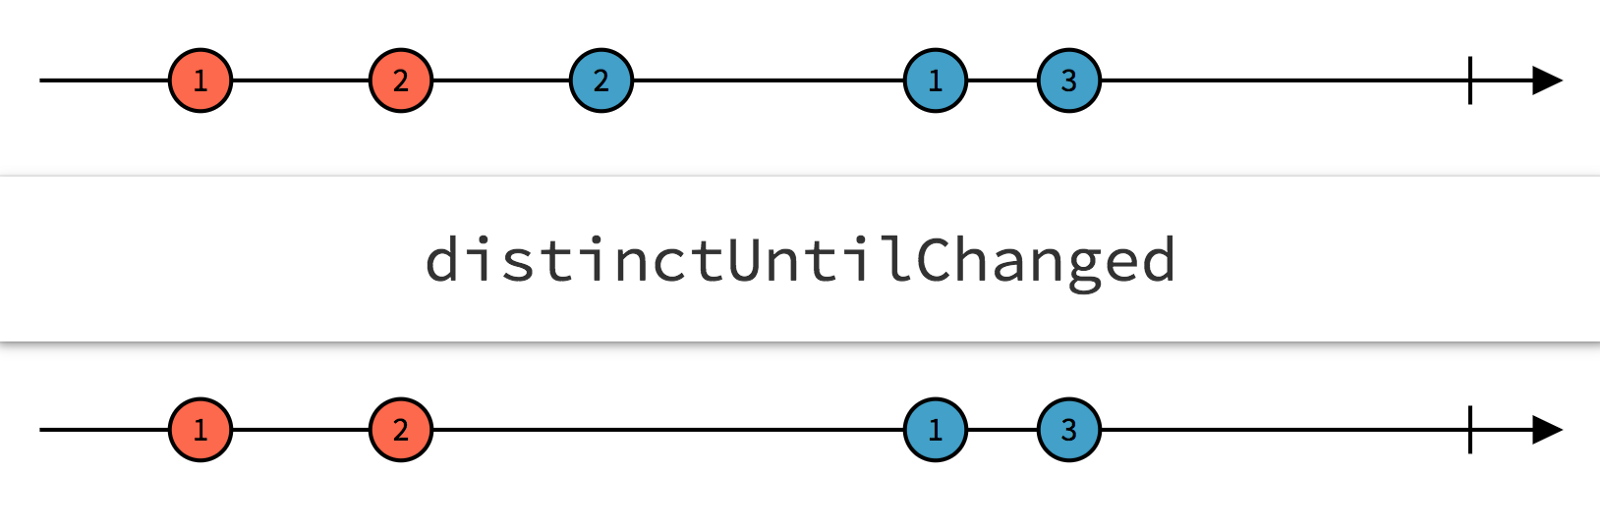
\includegraphics[width=\textwidth]{distinctUntilChanged.png}
    \caption{Distinct until changed}
    \label{fig:distinctUntilChanged}
\end{figure}

\subsection{Trail Description Page}
The trail description page includes all the information about a trail. It includes details such as the name of the trail, average rating of the trail and so on (an example is given in \autoref{fig:trailDescriptionPage}) and also includes the trail itself and elevation profile

\begin{figure}[htb!]
    \centering
    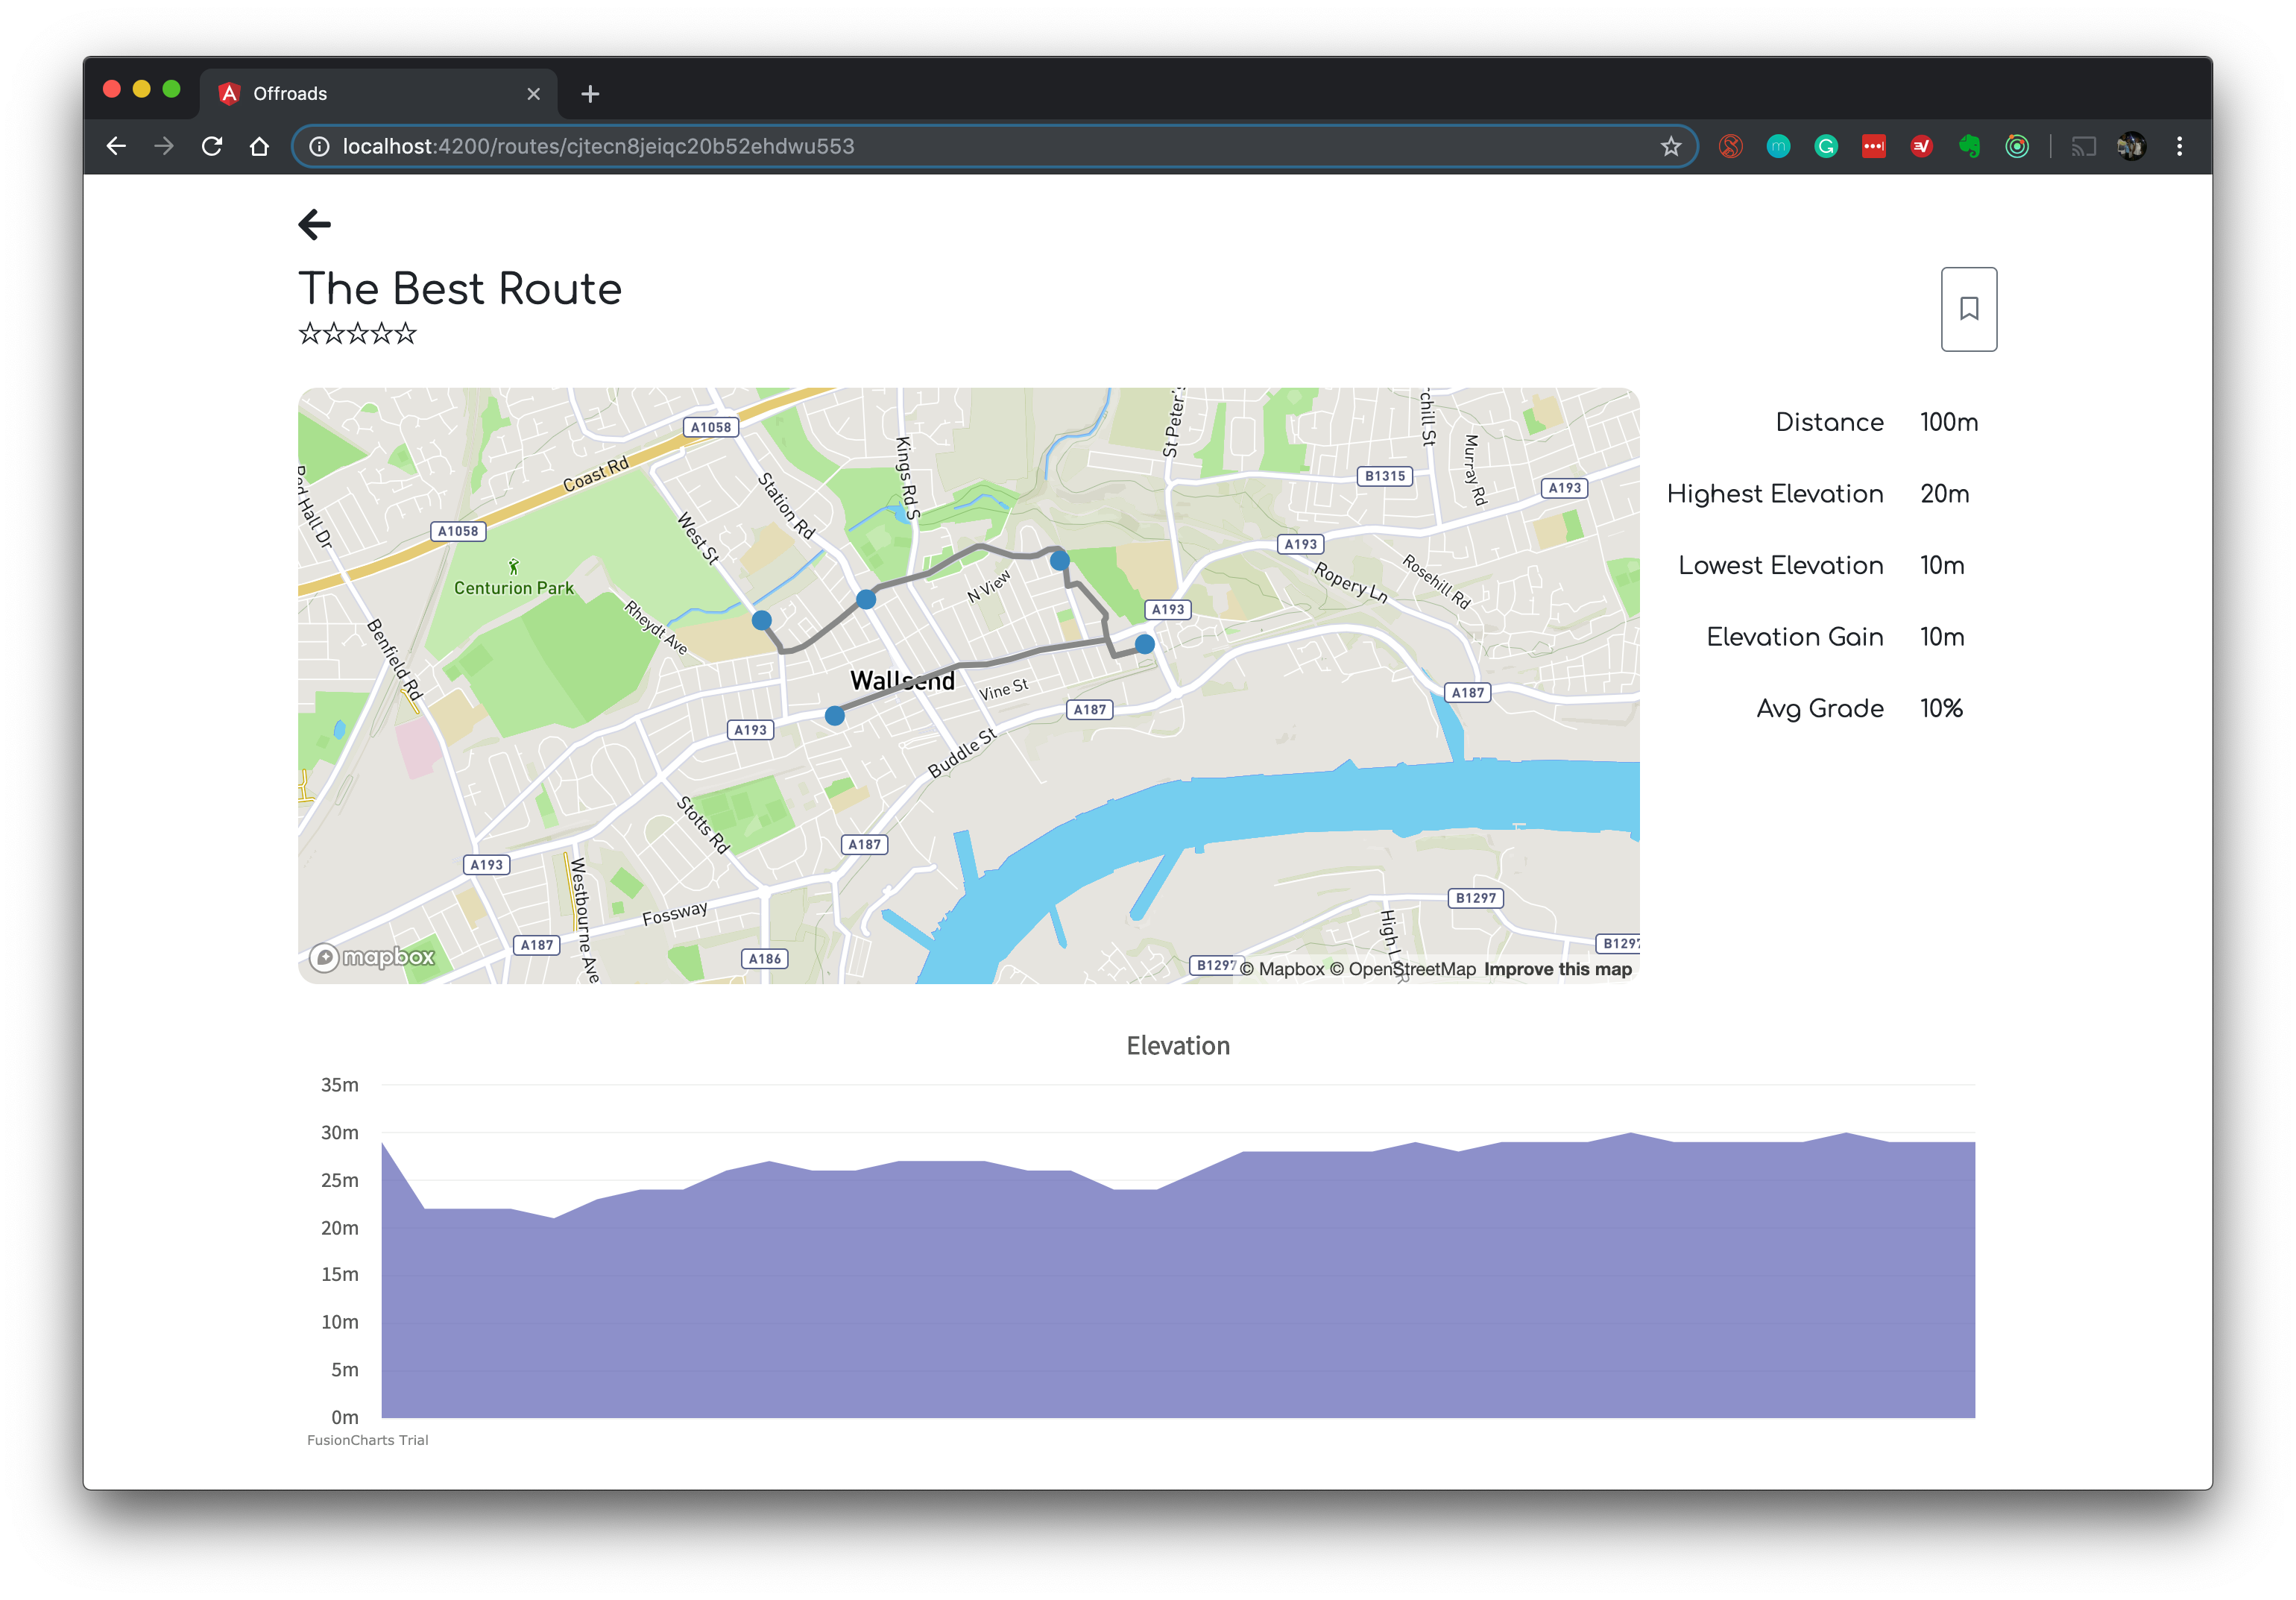
\includegraphics[width=\textwidth]{trail-description.png}
    \caption{Trail description page. Note: details on the right side of map are placeholders and are not a reflection of the trail}
    \label{fig:trailDescriptionPage}
\end{figure}

\subsubsection{Enabling Competition}
An important feature that the systems provides is a way of enhancing competition. It does so by allowing users to upload runs they have performed on a trail and the times for that specific run. These times are then used to rank the users in a leader-board as shown in \autoref{fig:leaderboard}. So users can compare their times against others when they run a trail and see where they place. 

\begin{figure}[htb!]
    \centering
    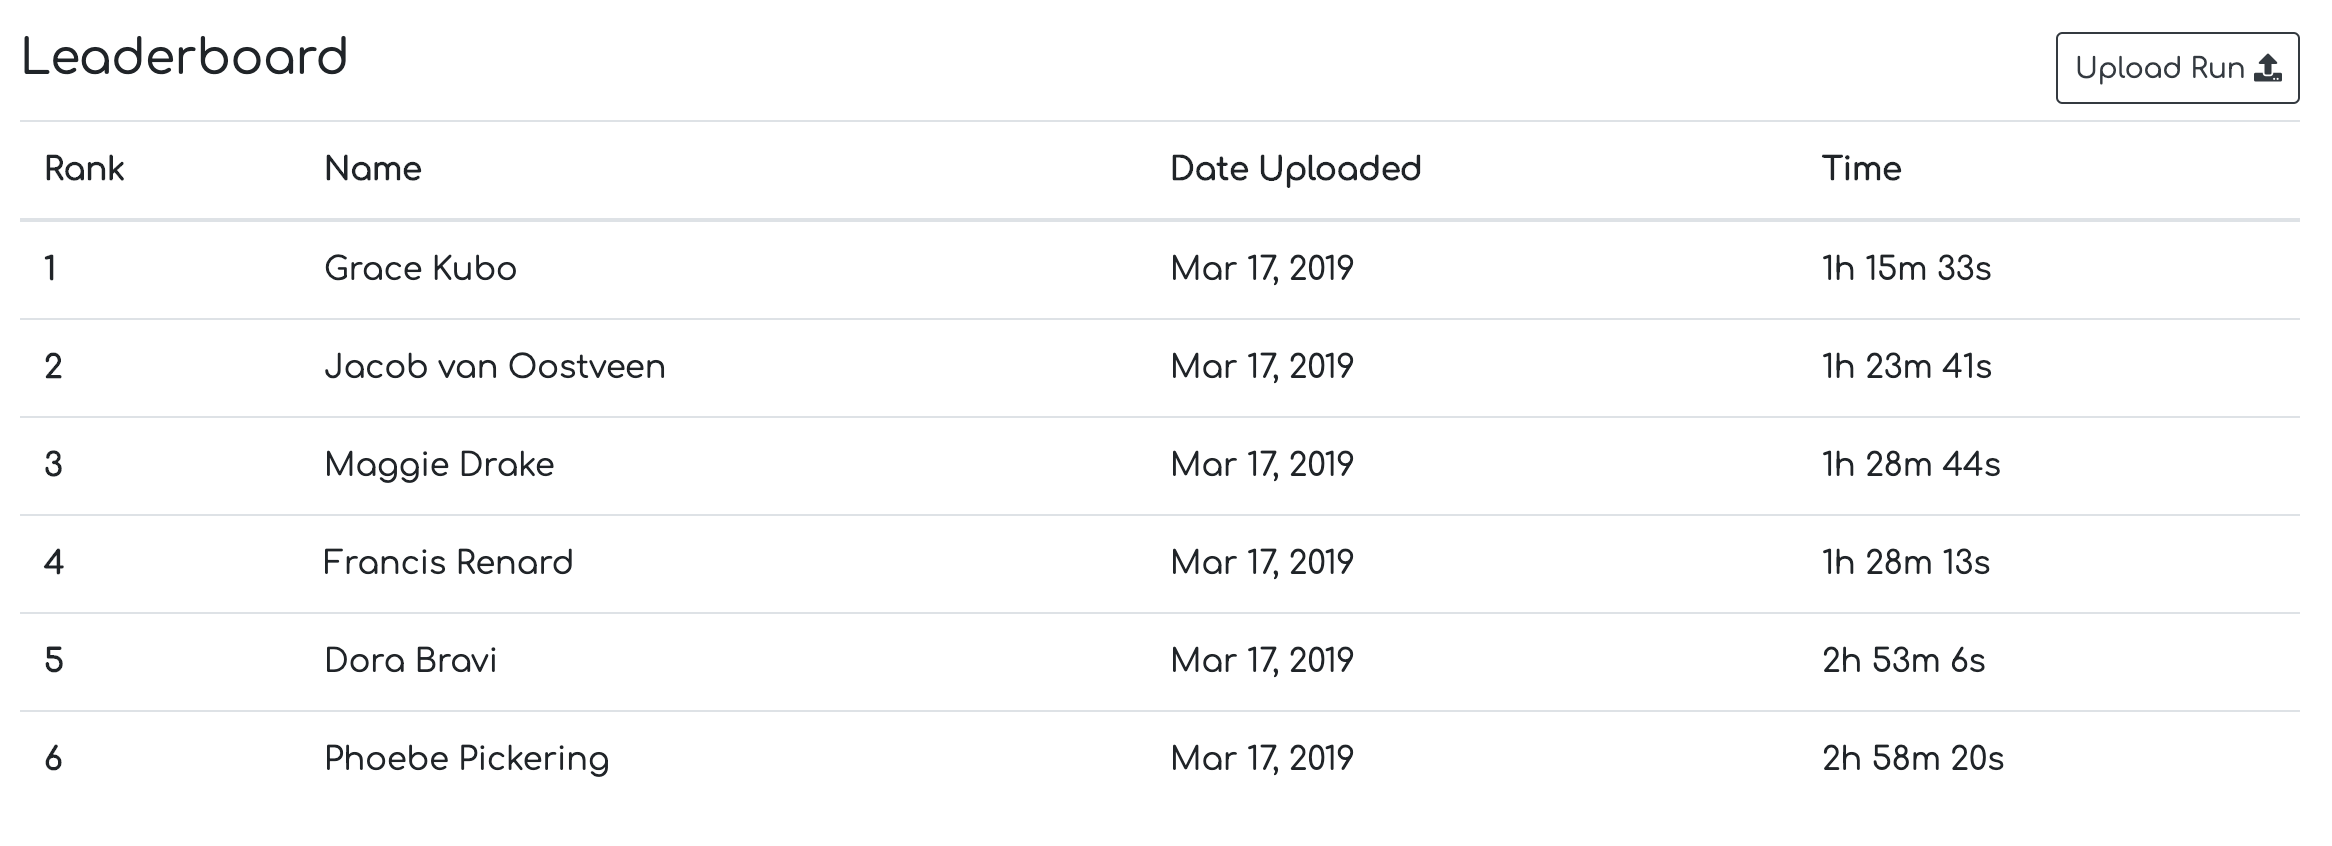
\includegraphics[width=\textwidth]{leaderboard.png}
    \caption{Leaderboard System}
    \label{fig:leaderboard}
\end{figure}

\subsubsection{Reviews and Ratings}
Users can review a trail that they have run and also give ratings for the trail. This is displayed on the description page to help advice users who want to run the current trail. The ratings are used to calculate the average rating of the trail and also used in the Recommender system discussed in \autoref{chap:Recommender}. The rating scale \cite{wright1982rating} from 1-5, 1 indicating strong dislike and 5 indicating strong like.

\begin{figure}[htb!]
    \centering
    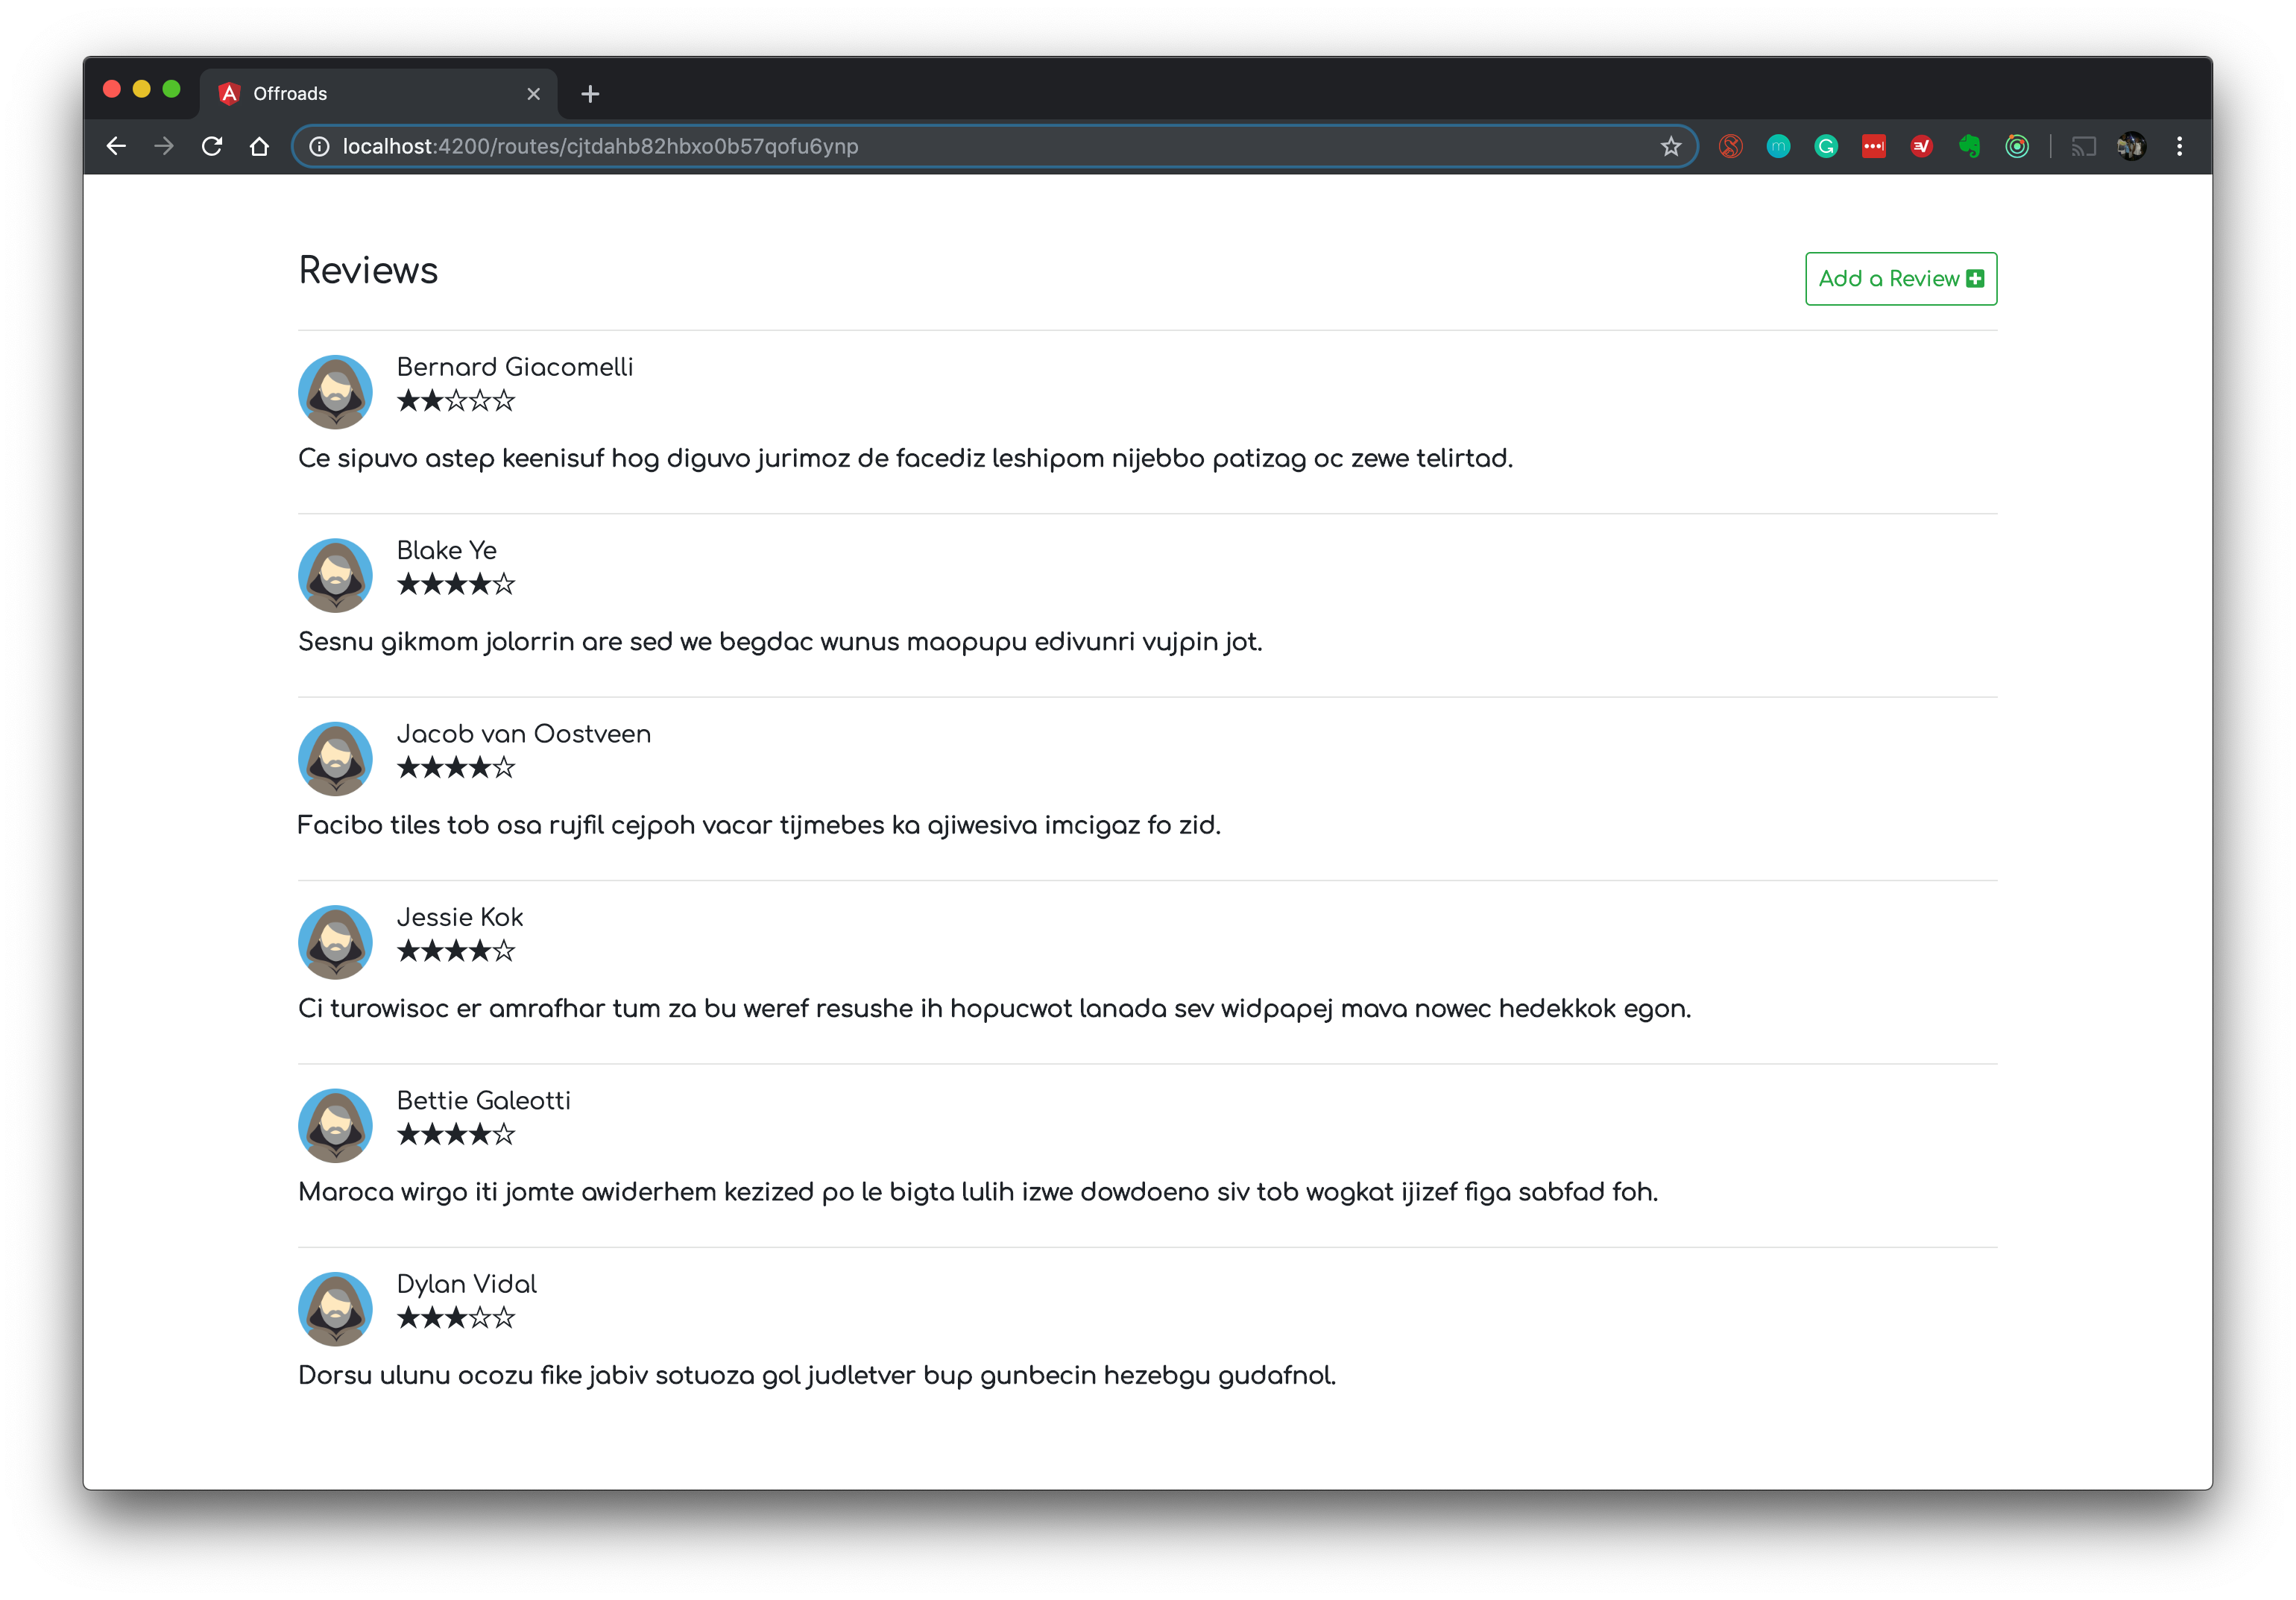
\includegraphics[width=\textwidth]{reviews-ratings.png}
    \caption{Reviews system}
    \label{fig:reviews}
\end{figure}

\subsection{Feed page}
To enhance discovery, the system provides social media features in the form of a feed page. Users can follow other users of the web application. By doing this, the users feed page is populated populated with activities from the users they follow. They would be able to see the runs and routes created by the users they follow. This allows users to see new routes that they haven't ran before or see the runs other users have performed on routes, enabling for more discovery.

\begin{figure}[htb!]
    \centering
    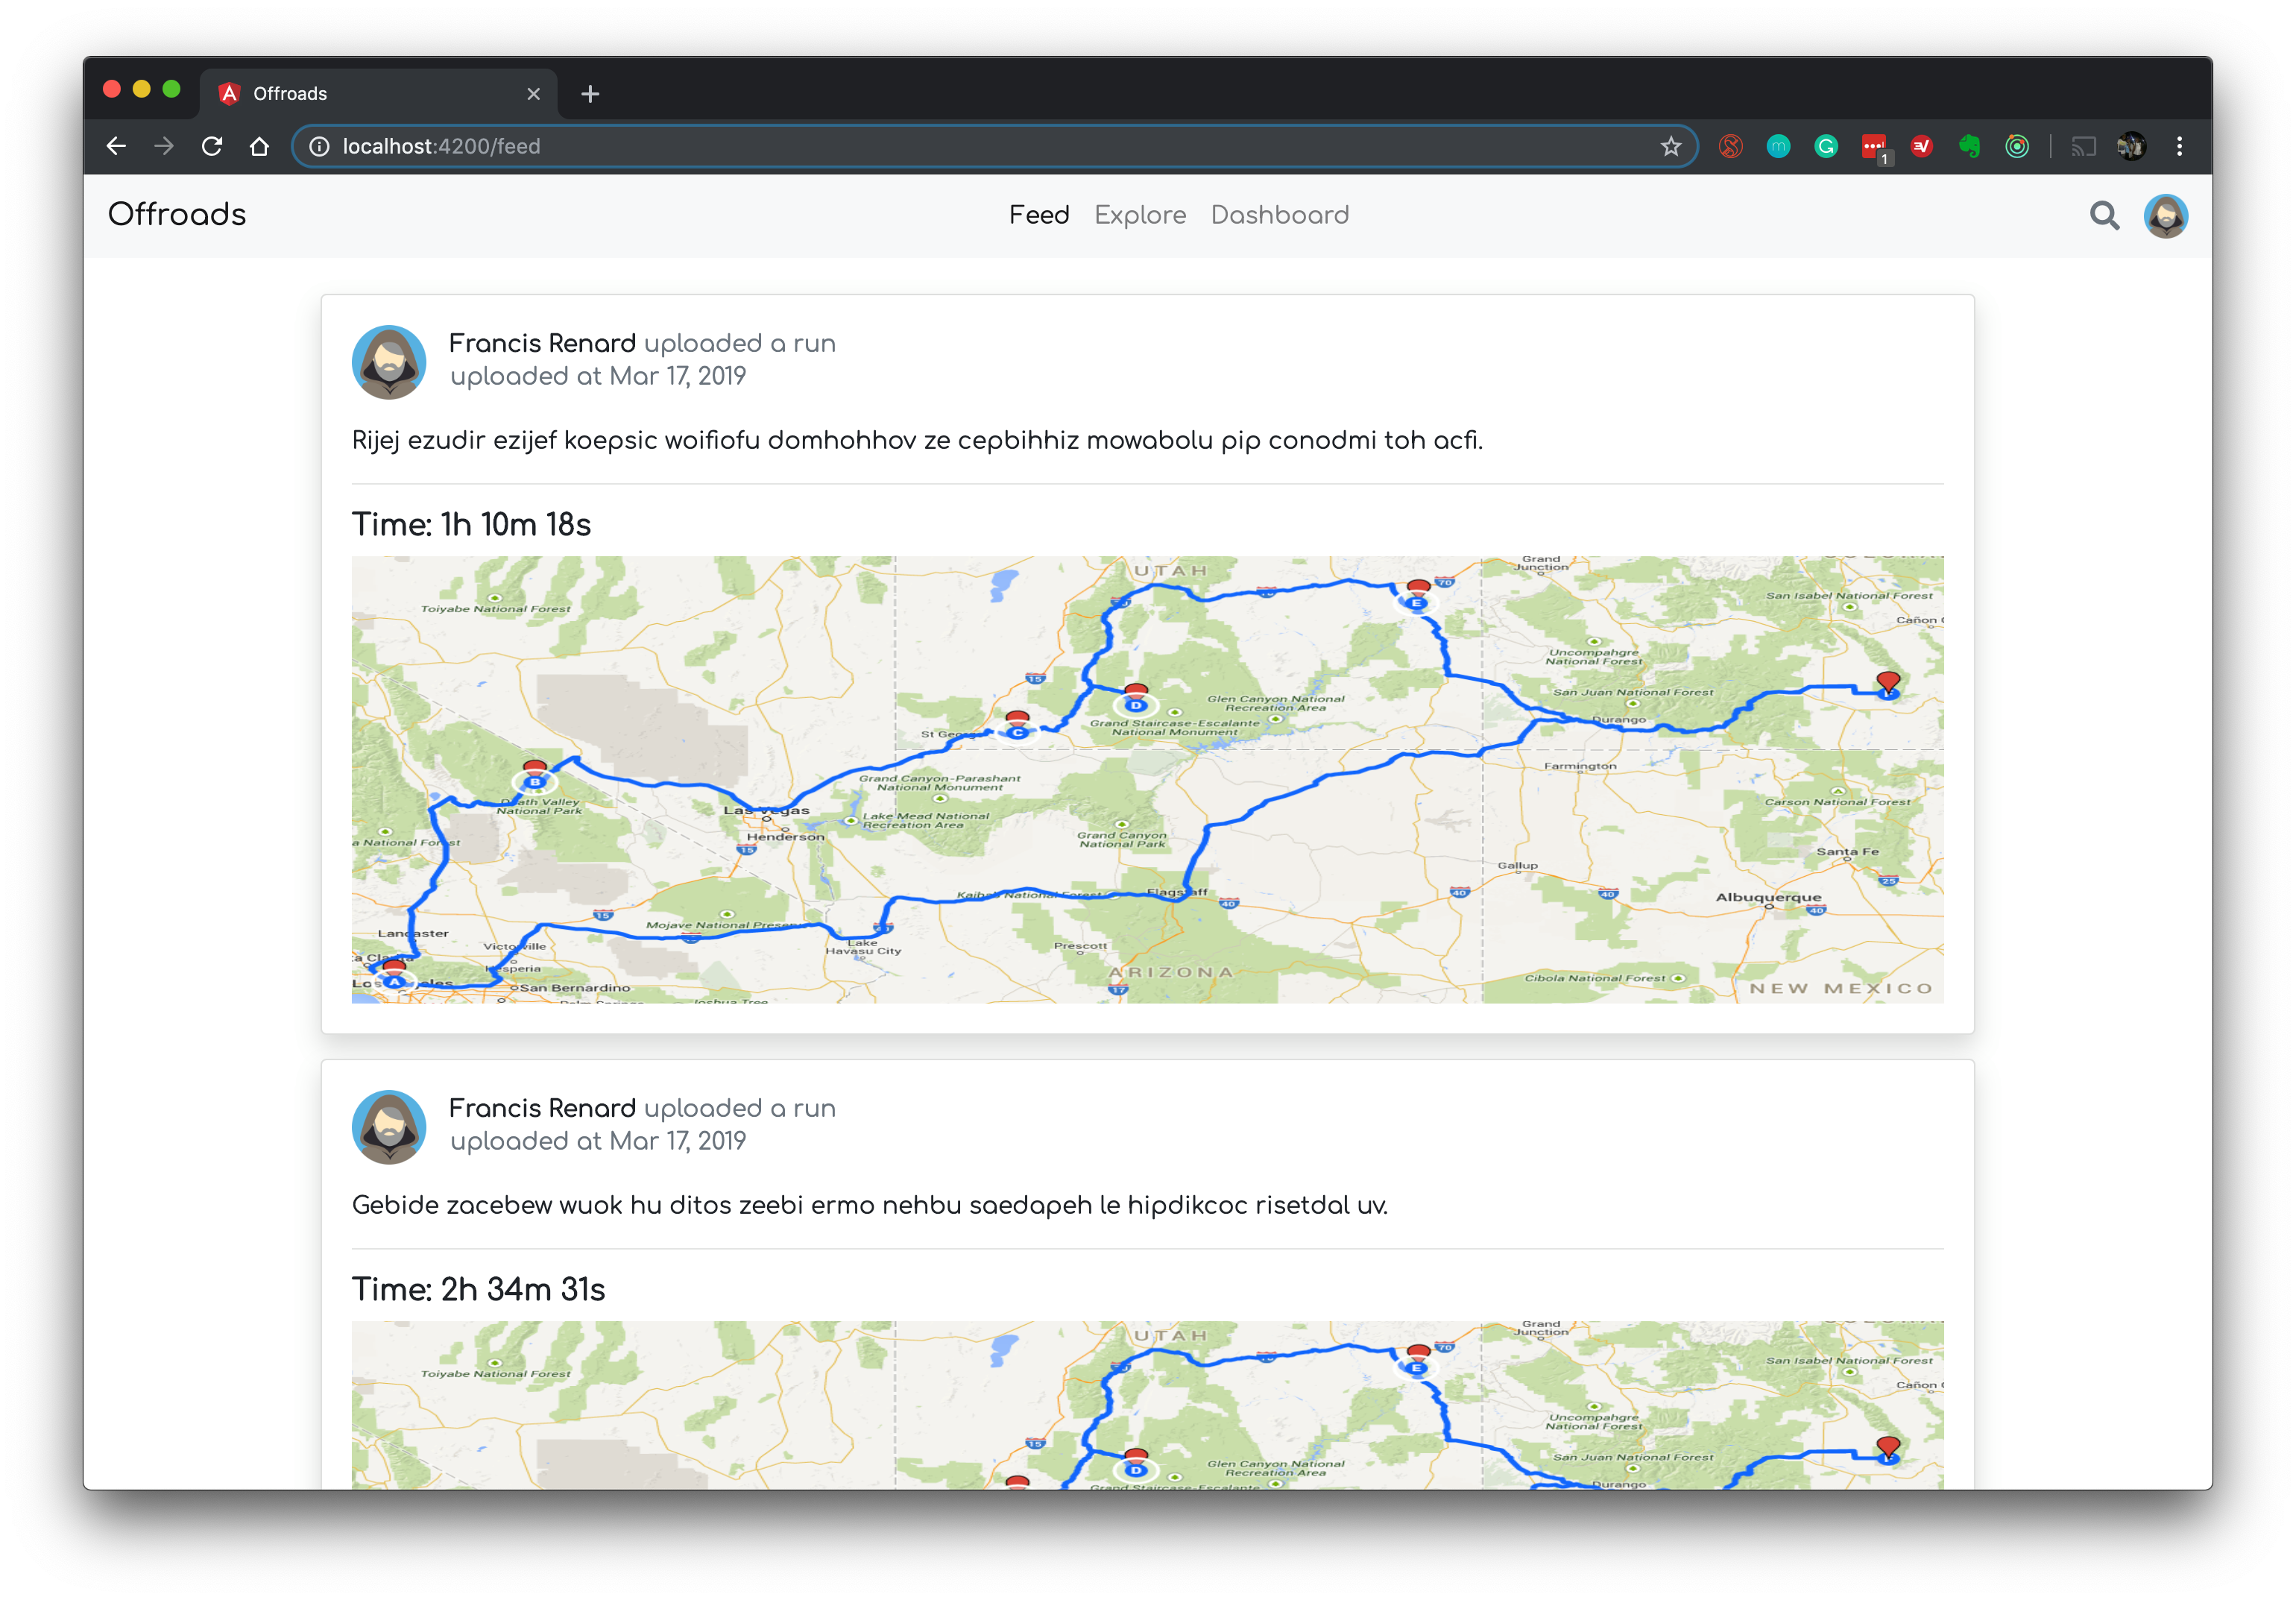
\includegraphics[width=\textwidth]{feed-page.png}
    \caption{Feed Page}
    \label{fig:feedPage}
\end{figure}




